\subsection{Sampling}

To select which models would perform the best with a specific set of hyperparameters along with ensuring a level of performance that is not just attributed to the luck of a chosen \texttt{random\_state}, there needs to be a repeated testing of the models' performance using different sets of data along with different sets of hyperparameters that modify how the models learn. For this, there is one main approach in dealing with consistency of performance and arbitrariness of choice: cross-validation.

\subsubsection{Train-test-split and Cross-validation}

Before cross-validation, a standard Train-Test-Split needs to prepend the sampling process. Consider the following example of simple k-fold cross-validation with 5 splits. The indices of the entries are within the range $[0, 100)$. table \ref{tab:kfold} shows the range of indices that would be within each fold:

\begin{table}[H]
    \caption{A simple example of a k-fold cross validation with a split/fold of 5 where the train and test columns show the index range of each set}
    \label{tab:kfold}
    \begin{tabularx}{\linewidth}{r|>{\centering}X>{\centering\arraybackslash}X}
        \toprule
        Fold & Test Set & Train Set\\
        \midrule
        1 & [0, 20) & [0, 100) - [0, 20)\\
        2 & [20, 40) & [0, 100) - [20, 40)\\
        3 & [40, 60) & [0, 100) - [40, 60)\\
        4 & [60, 80) & [0, 100) - [60, 80)\\
        5 & [80, 100) & [0, 100) - [80, 100)\\
        \bottomrule
    \end{tabularx}
\end{table}

While there are training and testing samples, they simply go on rotation for each fold. This would in turn feed the model all of the samples and train with all of them, this is something to take caution especially for grid search algorithms. For a grid search algorithm to be able to determine the best hyperparameters, it would need to perform a cross validation algorithm with each possible combination of hyperparameters. If the model would be trained and evaluated on all of the dataset, there is a sort of "leak" due to the hyperparameters actually being catered to what's best even for the testing data. For testing or predictions to be valid, it must be unbiased, and the best way to make sure of this is to make sure that the models never see the testing set that will be used to evaluate the models' performance. 

Hence, the traditional \texttt{train\_test\_split} algorithm was implemented. The algorithm would then train and evaluate itself by splitting the training of the dataset into smaller subsets of training and evaluating data. Refer to figure \ref{fig:tts cv} for a diagram illustrating the split, including the traditional \texttt{train\_test\_split} before the cross-validation (figure taken from \href{https://scikit-learn.org/stable/modules/cross_validation.html#cross-validation}{{\color{blue} scikit-learn page}}).

\begin{figure}[H]
    \centering
    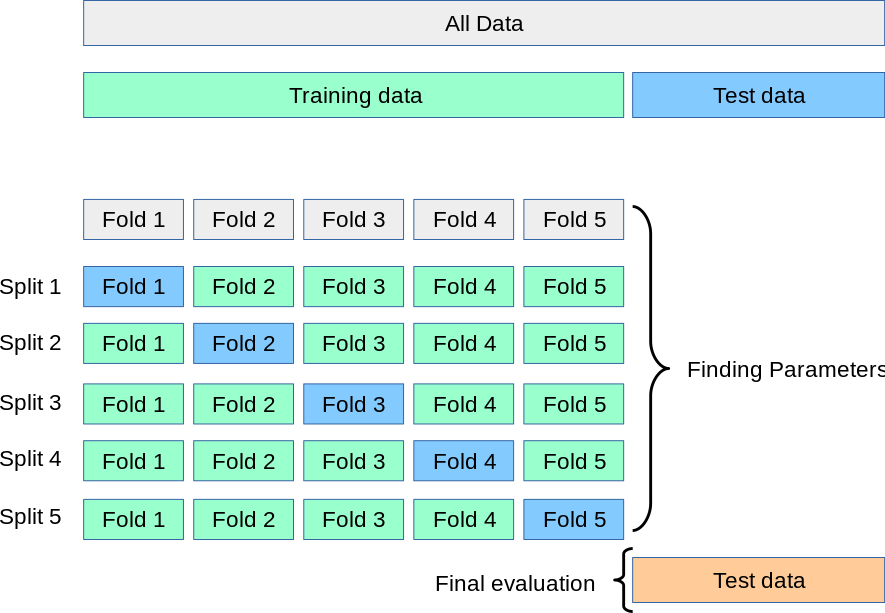
\includegraphics[width=\linewidth]{figures/grid_search_cross_validation.png}
    \caption{Illustration of the cross-validation folds after the initial train-test-split}
    \label{fig:tts cv}
\end{figure}

\subsubsection{GridSearch}

The \texttt{GridSearchCV} algorithm takes an input of hyperparameters and a cross-validation method. The algorithm would try all combinations of hyperparameters and test them with the cross-validation method to assess their performance. 
